% !TEX root = ../Thesis.tex
% !TEX spellcheck = en-US

\chapter{Introduction}
\label{ch:introduction}

This first chapter introduces the challenge of using virtual, fully software-based alternatives to computer network labs in education, with special emphasis on the undergraduate and graduate levels of the university. % TODO should university by capitalized here?
It also proposes the definitions that, though not universal or unique, help precise differences between those software solutions, namely two main concepts: simulation and emulation. % TODO universal NOR unique?
Together with the last point, this chapter also explains the reason why this thesis is centered, starting from its title, in ``emulators'' more than on ``simulators''.
Finally, it gives a very brief overview of the work that has already been done in the field of computer networks simulators and emulators, and, orthogonally, in the replacement of laboratories with (physical) hosts and routers/switches in schools and universities by simulated or emulated (virtual) solutions.

% end of intro

\section{Motivation and problem statement}
\label{sec:motivation}

\subsection{The lab on a laptop}
\label{subsec:replacingthelab}

% end of subsec replacingthelab

\subsection{Emulation, simulation (and virtualization)}
\label{subsec:emulsimvirt}

% end of subsec emulsimvirt

% end of section motivation

\section{Related work}
\label{sec:relatedwork}

% PROBABLY SOME SUBSECTIONS GO HERE

% \subsection{The lab on a laptop}
% \label{subsec:replacingthelab}

% % end of subsec replacingthelab

% \subsection{Emulation, simulation (and virtualization)}
% \label{subsec:emulsimvirt}

% % end of subsec emulsimvirt

% end of section gns3performance

\begin{figure}
  \centering
  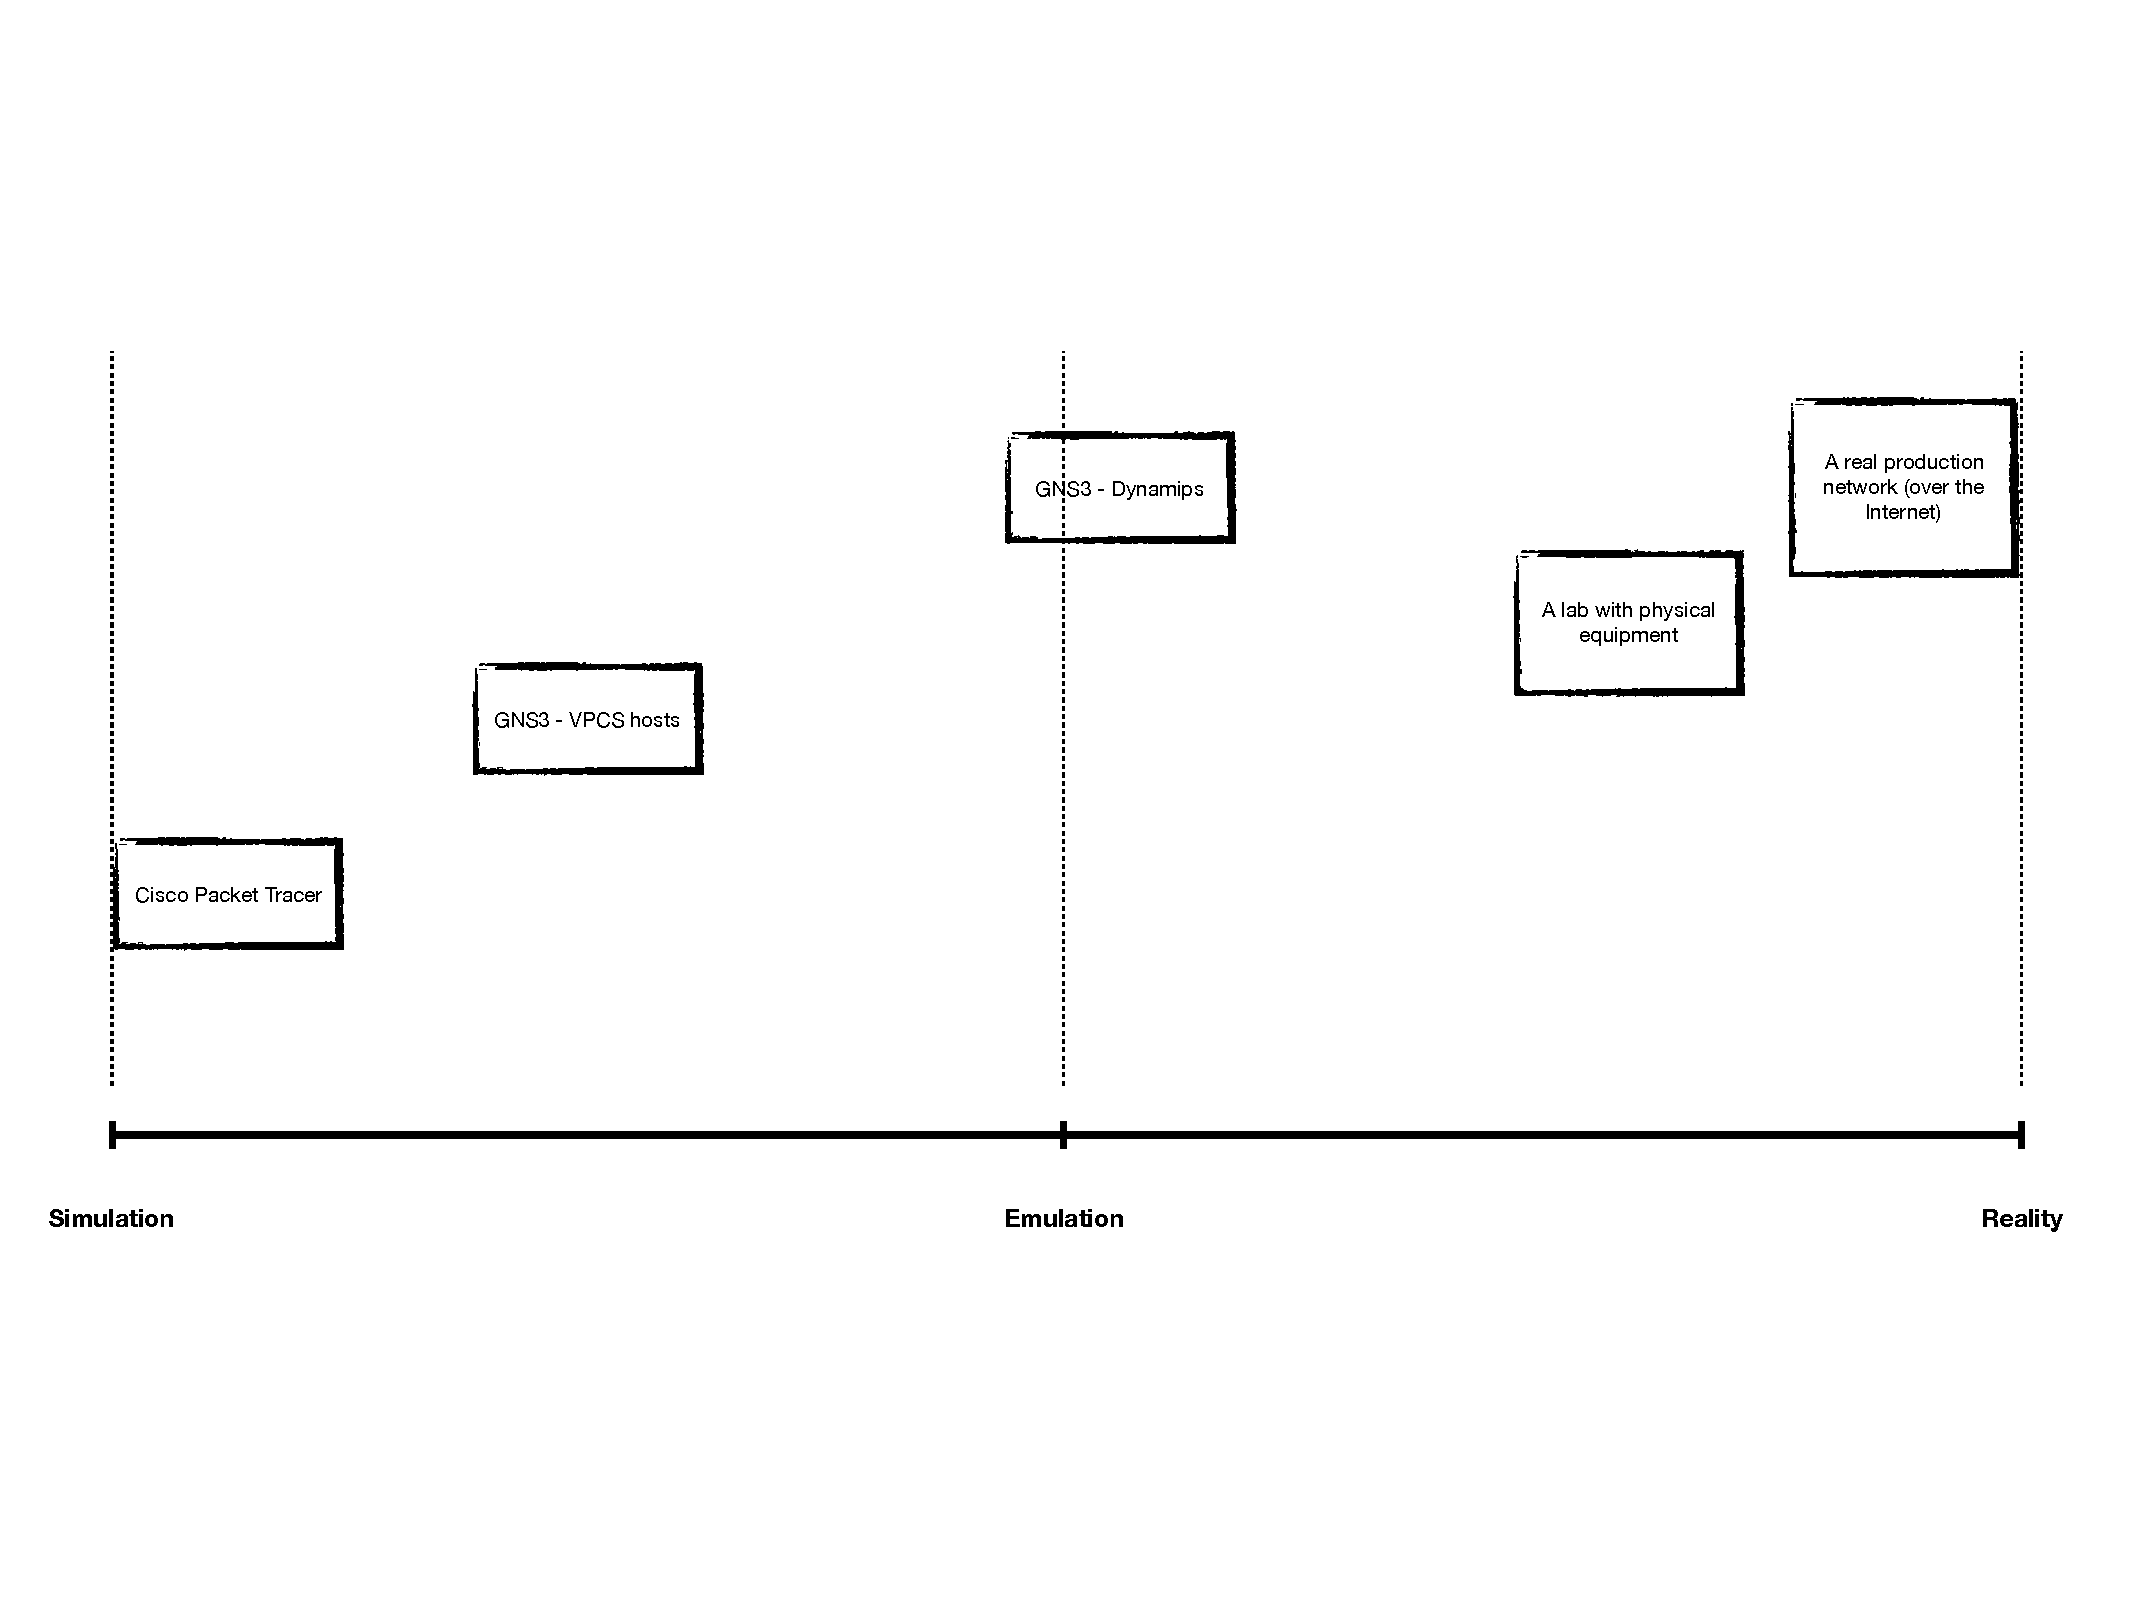
\includegraphics[width=0.8\textwidth]{emulationvsreality}
  \caption{Simulation vs emulation vs reality}
  \label{fig:emulationvsreality}
\end{figure}

% \section{The first section of this intro}
% Here we can comment on the super-interesting aspects of the diagram depicted in figure~\ref{fig:emulationvsreality}.

\section{Structure of the thesis}
\label{sec:structure}

% end of section structure

% end of chapter
